\section{Introduction} \label{sec:intro}


Remote sensing technology is an essential resource for Earth observation, offering the possibility to work on a large scale with cheap, reasonably accurate, and faster results compared to ground-based methods.

Land Surface Temperature (LST) images are of prime importance to efficiently monitor physical processes related to climate change, such as water stress, evapotranspiration, wildfire risk, or urban heat islands \cite{lst2005}.
Additionally, LST has been approved as a high-priority parameter for the International Geosphere and Biosphere Program (IGBP) \cite{townshend94}. LST is retrieved from remote sensing images in the Thermal infra-red (TIR) spectral domain. 

Some of the applications mentioned above have very exigent requirements for TIR data products, requiring as many detailed images as possible (spatial resolution) and having many images available per day (temporal resolution) to monitor the dynamic processes involved.
The currently available products do not meet these requirements, and the lack of data may hinder research.

Upcoming satellite missions such as SBG, Trishna, and LSTM will join forces to provide a 50m GSD product at daily revisit \cite{author2023thermal}. However, their joint system will not be available until the end of the current decade, assuming no further delays. Additionally, applications like urban heat require more than one image per day.
Private satellite providers such as OroraTech are deploying cubesat (small satellites) constellations that provide high temporal resolution. Still, their smaller payload generally results in a lower spatial resolution that is insufficient for local scale applications and fine-scale analysis, especially in highly heterogeneous environments like urban areas, diverse agricultural plots, or sparse forests.

Super resolution (SR) is a post-processing technique that aims to increase the spatial resolution of images while preserving their physical consistency.
Using artificial intelligence (AI) for SR has many applications in heterogeneous fields like medical imaging, computer vision, and remote sensing. Several deep learning architectures have been proposed with promising results, but applying them to real data remains a challenge. 
Super resolution is a supervised task that typically requires paired high-resolution (HR) and low-resolution (LR) images, something that is challenging to acquire in real-world applications. To circumvent the issue, synthetic datasets are created by obtaining HR images and intentionally degrading them. The term ``degradation'' refers to artificially reducing an image's quality and simulating an LR version from it, commonly achieved using a degradation model consisting of Gaussian blurring kernels and additive white noise. However, this might not accurately represent real-world degradation's complexities and specific characteristics in satellite imagery.

This thesis will focus on enhancing the resolution of TIR data products from OroraTech's FOREST-2 mission to improve their LST products and facilitate research progress. The study is centered around the following key research questions:

\begin{itemize}
    \item What is the impact of the unknown FOREST-2 degradation model compared to the one commonly used for dataset generation?
    \item Is it possible to estimate the FOREST-2 degradation model using a data-driven approach?
    \item How can the degradation model be incorporated into training to improve SR results?
    \item  How can the SR results be assessed when paired data is scarce?
\end{itemize}

Considering these questions, a framework that allows SR for low spatial resolution TIR data products from any mission will be proposed without the need for paired data.
 
In Chapter 2, a brief introduction to remote sensing and LST retrieval is presented alongside the different quality dimensions of remote sensing data. The motivation for this work is introduced in Chapter 3, diving deeper into applications of TIR data and their requirements. The trade-off between spatial and temporal resolution of the currently available products is also shown.

The main techniques of super resolution are summarized in Chapter 4, as well as the main challenges in dataset generation techniques used in the literature.
The domain gap problem is also explained, as well as the concept of blind super resolution.

In Chapter 5,  the methodology of this work is presented, including the model architecture and the rationale behind the selection. Additionally, the degradation models used to obtain a baseline model and the metrics used for evaluation are discussed.

In Chapter 6, the data gathering process is introduced, and the datasets used in the experimentation are presented along with the assumptions made to generate them.

The experimentation setup is introduced in Chapter 7, including the training parameters and heuristics to select the best models.

Chapter 8 presents a thorough analysis of the experimental results, and chapter 9 builds on it, offering the conclusions of the work and possible future research directions.

\newpage

    
\section{Thermal Remote Sensing} \label{sec:thermal_remote_sensing}

In general terms, remote sensing is the science and practice of acquiring information about an object without actually coming in contact with it.
Remote sensing is a technology for sampling reflected and emitted electromagnetic (EM) radiation from the Earth's terrestrial and aquatic ecosystems or the atmosphere.
This is typically done by recording images from airplanes and satellites to help identify or better understand features on the Earth's surface.

A simple example of a remote-sensing instrument is a photographic or digital camera.
The instrument records energy through light reflected from a surface to form an image.
Most photographic cameras record visible light so that the image resembles the photographed feature, but more sophisticated remote-sensing instruments can record energy outside of the range of visible light.
Data from remote-sensing instruments can be recorded as images or, in other cases, such as lidar, a series of point data.

    \subsection{Electromagnetic spectrum}

    The electromagnetic spectrum (EMS) includes wavelengths of electromagnetic radiation ranging from short wavelength (high frequency) gamma rays to long wavelength (low frequency) radio waves. 
    Most applications focus on the spectrum region, starting in the ultraviolet and continuing through the microwave wavelengths. 
    Optical sensors are used to measure ultraviolet, visible, and infra-red wavelengths, while microwave sensors are used for the microwave portion of the EMS.
    
    A fundamental physical principle that remote sensing relies on is that different features on the Earth's surface interact with specific wavelengths of the EMS in different ways.
    When working with optical sensors, the essential property used to identify features on the Earth's surface is spectral reflectance, the ratio of light reflected from a surface divided by the intensity of incident light.
    Different materials have different spectral reflectance properties, and this information can be used to identify individual features.
    For example, white sand reflects visible and near-infra-red light, whereas green vegetation absorbs most red wavelengths and reflects the most near-infra-red wavelengths.    

    Unlike the visual spectrum, the emitted light is measured in the infra-red spectrum (IR).
    This is because all bodies have a temperature above absolute zero, which can be detected as radiation.


    The IR spectrum goes from 1400 nm wavelength to 1 mm and is further subdivided due to its width:


    \begin{itemize}
        \item  Short-wave infra-red (SWIR): 1,4 to 3,0 µm
        \item  Medium-wave infra-red (MWIR): 3,0 µm to 8 µm
        \item Long-wave infra-red (LWIR): 8 to 15 µm
        \item Far-infra-red (FIR): 15 µm to 1000 µm
    \end{itemize}

    \begin{figure}[H]
        \centering
        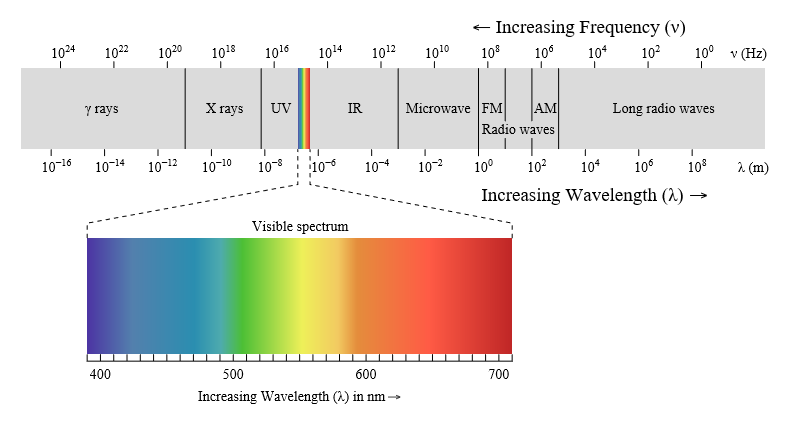
\includegraphics[width=\textwidth]{Includes/1-electromagnetic-spectrum.png}
        \caption{Electromagnetic spectrum}
        \label{fig:1-electromagnetic-spectrum}
    \end{figure}


    
    Like in the visual spectrum, TIR information is obtained in a purely passive way.
    Thermal infra-red detectors called bolometers are primarily used on drones or ground stations due to their small volume, weight, and energy consumption. 
    They offer a low accuracy in relative and absolute temperature measurement and are relatively inert. However, they are worthwhile for aircrafts with small payload capacity.     
    More complex systems are cooled to cryogenic temperatures to reduce thermal noise, a random electronic fluctuation whose power is proportional to the temperature that can interfere with the signals. The noise reduction allows the sensor to have higher sensitivity and accuracy. In contrast to bolometers, they are significantly larger and require more energy, making them unsuitable for drone use. This type of detector is used on all standard TIR satellite systems.

    \subsection{Land surface temperature}


        Land Surface Temperature (LST) is the radiative temperature of the land, derived from the previously mentioned thermal infra-red radiation that the Earth's surface emits. It is a crucial parameter affecting surface energy balance, regional climates, heat fluxes, and energy exchanges.
        When measuring Earth's temperature, the interest relies on (TIR) specifically, which has a wavelength of 3 to 14 µm (both MWIR and LWIR), corresponding to black body temperatures of between -60°C and 700 °C, according to Planck's law.

        \begin{equation}
            B_{\lambda}(T) = \frac{C_1}{\lambda^5 \left[ \exp\left(\frac{C_2}{\lambda T}\right) - 1\right]}
        \end{equation}

        Where $B_{\lambda}(T)$ is the spectral radiance, $C_1$ and $C_2$ are constants, and $\lambda$ is the radiation wavelength. 
        Accurate LST retrieval from TIR data depends on atmospheric effects, sensor parameters such as spectral range and viewing angle, and surface parameters such as emissivity and geometry. Many researchers have proposed different approaches for LST retrieval, considering these factors.
        These algorithms are named considering the number of TIR bands used. For instance, single-channel or mono-window algorithms use one TIR band. However, split window or multi-channel methods include more than one TIR band. Some examples of these methods are Single Channel Algorithm (SCA) \cite{sca2009} and Mono Window Algorithm (MWA) \cite{mwa2001}. The reader is referred to \cite{LI201314} for a more detailed review.


        A straightforward way to retrieve LST from a TIR band is inverting the simplified radiative transfer equation (RTE) \cite{becker90}. This equation contemplates that the radiance measured by the sensor is a combination of the emitted radiance from a surface that is not a blackbody, the reflected radiance from the atmosphere, and the radiance emitted by the atmosphere itself.


        \begin{equation}
            \begin{aligned}
            L_{sensor} &= \left[ \varepsilon \cdot B_{\lambda}(T) + (1 - \varepsilon) \cdot L_{atm}^{\downarrow} \right] \tau + L_{atm}^{\uparrow} \\
            B_\lambda (T) &= \frac{L_{sensor} - L_{atm}^{\uparrow}- \tau (1 - \varepsilon) \cdot L_{atm}^{\downarrow}}{\varepsilon \tau} 
            \end{aligned}
        \end{equation}

        Where $L_{sensor}$ is the radiance measured by the sensor, $\varepsilon$ is the surface emissivity, $B_{\lambda}(T)$ is the Planck law equation, $L_{atm}^{\downarrow}$ is the downwelling path atmosphere radiance and $L_{atm}^{\uparrow}$ is the upwelling path atmosphere radiance. 
        The temperature can then be obtained from the spectral radiance:

        \begin{equation}
            T = \frac{C_2}{\lambda \cdot \log\left(\frac{C_1}{\lambda^5 \cdot \left[ \frac{L_{sensor} - L_{atm}^{\uparrow}- \tau (1 - \varepsilon) \cdot L_{atm}^{\downarrow}}{\varepsilon \tau}  \right]}+1\right)}
        \end{equation}

        From all the inputs for LST retrieval, radiance is the only one not available in high resolution, making it the bottleneck for the task. The high LST and TIR resolution dependency makes them particularly interesting for this work.
        
       

    \subsection{Quality dimensions of remote sensing data}

    Remote sensing data can be characterized by four quality dimensions, as stated in \cite{HORNING20082986}:

    \begin{itemize}
        \item Spatial resolution: This is often referred to as resolution and is the size of a pixel in ground dimensions. 
        In most cases, an image's resolution is labeled with a single number, such as 30 m, representing the length of a side of a square pixel if it were projected onto the Earth's surface.
        If the pixel were rectangular, then the length and width of the pixel would be provided.
        \item Spectral characteristics: This includes bandwidth, band placement, and the number of bands.
        Spectral bandwidth, or spectral resolution, refers to the range of wavelengths detected in a particular image band.
        This effectively measures how precisely an image band measures a portion of the EMS.
        Band placement defines the portion of the EMS that is used for a particular image band.
        For example, one band might detect blue wavelengths, while another might detect thermal wavelengths along the EMS.
        The last spectral variable is the number of bands. The more bands that are available, the more precisely the spectral properties of a feature can be measured.
        \item Acquisition dynamics: This dimension has two components. The first is the minimum time a particular feature can be recorded twice, often called the revisit time or temporal resolution.
        Some sensors with a vast field of view can acquire multiple images of the same area on the same day, whereas some sensors have a repeat frequency of several weeks.
        The other component is the timing of the acquisitions. 
        Dynamic features such as forests shedding leaves in autumn and events such as flooding often have an optimum time for which they should be imaged.
        For example, identifying deciduous vegetation is aided by acquiring imagery during leaf-on and leaf-off periods.
        \item Sensitivity of the sensor: This is defined by the dynamic range of the sensor as well as the range of digital numbers that can be used to represent the pixel values.
        Sensors have lower limits below which a signal is not registered and upper limits above which the sensor saturates and cannot measure increases in radiance.
        The detail that can be measured between these extremes is determined by the range between the minimum and maximum digital numbers permitted for a particular data type.
        This potential range of values is often called quantization or radiometric resolution.
    \end{itemize}
    
    
    \newpage
    

\section{Motivation}

Unlike ground-based methods, satellites can continuously monitor vast tracts of land regardless of smoke or geographical barriers, providing critical data that can significantly enhance early detection and response efforts. 
However, while current satellite systems offer extensive spatial coverage and consistent data collection, they are not without limitations, particularly in the quality dimension of spatial and temporal resolution. Throughout this section, some applications for LST data will be presented, as well as the thermal data product requirements that the literature has identified as vital for their development. The trade-off between spatial and temporal resolution that current available products have will be further discussed.
    

    \subsection{Wildfire Monitoring}

    Forest fires can be natural or human-generated phenomena that occur in natural ecosystems and usually spread uncontrollably.
    They have increased steadily worldwide over the past decade, and according to the UN Environment Programme (UNEP), this trend will continue, with a potential 50\% increase by the end of the century \cite{UNEP2021Wildfire}. 
    The escalating frequency and intensity of wildfires across the globe have prompted a reassessment of current monitoring systems and methodologies. Traditional ground and aerial surveillance methods are proving inadequate in the face of rapidly spreading, unpredictable fires, particularly those obscured by smoke and difficult terrain. This inadequacy hinders effective firefighting efforts and exacerbates these disasters' environmental, economic, and human toll. 
    In most cases, a fume layer is not an obstacle for a satellite to detect a fire, as they rely on thermal infra-red sensors that can measure radiance through the smoke.

    Prevention is the most effective way to fight wildfires, and early detection is vital for achieving this goal. 
    With timely access to thermal data from space, potential wildfires could be identified before they spread, minimizing damage and saving lives.
    Although emergency response agencies use satellite-based imagery to monitor large-scale wildfires that burn over extensive periods, the wait interval for a satellite overpass induces a considerable time delay, which prevents its application in time-sensitive fire detection scenarios, such as emergency evacuations, early detection or search-and-rescue operations \cite{lippitt2015time}. 

    Wildfire management and insurance companies also leverage remote sensing for fire risk mapping, modeled as the combination of the fire probability, its behavior, and its effect \cite{crichton99}. Correctly estimating the likelihood of ignition events can help insurance companies charge accurate prices, and wildfire managers perform actions like controlled burns to reduce imminent risk. 
    Having risk ratings at a property level would give both industries the spatial granularity they need to improve their products. Additionally, short-term fire risk maps require high temporal resolution data to rapidly adapt and update the dynamic parameters they use as input \cite{rs11222638}.


    OroraTech seeks to circumvent the overpass wait time issue by launching a swarm of small satellites that have been especially helpful for detecting newly born fires that started as a result of a more extensive fire spreading, burning the material around its vicinity. Beginning in 2026,  the team will deploy sensors capable of providing up-to-date thermal data of the entire Earth every 30 minutes. However, as seen above, another vital parameter to measure fire risk, detect burn areas, and monitor vegetation recovery is the spatial resolution. The coarse spatial resolution of these satellites' smaller payloads does not enable the reliable detection of smaller fires or map risk at the required level. Additionally, higher spatial resolution is needed to better estimate the firefront, which is vital for the emergency response teams to plan their actions.
    Moreover, HR data has been used to validate characteristics of false positives in fire detection algorithms applied to LR images \cite{ijgi11120601}. 

    \subsection{Urban heat}

    Productivity losses due to heat currently cost an estimated \$100 billion annually in the US alone.
    The UK experienced unprecedented temperatures, too, temporarily knocking out services for giants like Google and Oracle and further affecting their clients.
    These are only a few examples of how businesses are affected by extreme temperatures in urban areas \cite{atlanticcouncil2021extreme}.  

    Public interest and concern about heat waves are steadily rising, especially in moderate climate areas like North Europe. Heat waves pose a significant threat, especially to vulnerable populations, including older people who are more susceptible to heat stress, pregnant individuals struggling to adapt to temperature changes, outdoor workers who are exposed to extreme heat for prolonged periods, and low-income neighborhoods with poor-quality buildings, among others \cite{Hsu2021Disproportionate}.   

    Urban heat refers to the phenomenon where urban areas experience higher temperatures than their more rural surroundings.
    This effect can be attributed to various factors such as building geometry, thermal properties of building materials, radiation properties of surfaces, and anthropogenic heat release from sources such as traffic and industry \cite{deilami2018urban}. 
    In particular,  the Urban Heat Island (UHI) phenomenon refers to the air temperature differences between urban areas and their surrounding rural regions, typically most pronounced during the evening and night hours. 

    Monitoring the UHI effect traditionally involves recording measurements from meteorological stations in urban and rural regions.
    However, an alternative method is to use thermal remote sensing, which allows the monitoring of large areas without the need for multiple physical sensors placed throughout the city.
    Research suggests that a Ground Sampling Distance (GSD) of 50m to 100m is the minimum spatial resolution requirement for urban thermal environment studies \cite{mohamed2017land, sobrino2012impact, huang2013generating}. 
    These conditions can be met by missions such as Landsat \cite{USGS2023Landsat} and Terra \cite{terra_nasa}, which provide a high spatial resolution in the thermal infra-red band.
    However, their weekly revisit time severely limits the analysis of dynamic processes with a temporal resolution in the order of hours, such as the UHI. 

    Existing studies on the UHI effect have been limited by the low spatial resolution of the images used and the lack of satellite images available at different times of the day \cite{Zhu2021, Shi2019}. 
    In particular, researchers explicitly state their limitations \cite{Shi2019} due to the low frequency of revisits while studying the Park Cool Island (PCI) \cite{Yang2017} phenomenon. 
    The influence of vegetation cover on the UHI phenomenon has been recognized as the foremost determinant \cite{deilami2018urban}, where parks have been found to exert a cooling impact.
    Fig. \ref{fig:1-skopie-UHI} illustrates an example that demonstrates this influence. 
    
    \begin{figure}[H]
        \centering
        \begin{minipage}{0.75\textwidth}
            \centering
            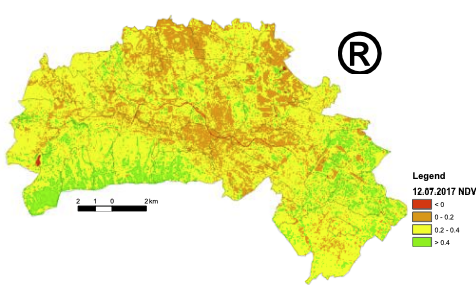
\includegraphics[width=\textwidth]{Includes/1-skopje-NDVI.png}
            \label{fig:1-skopje-NDVI}
        \end{minipage}\hfill
        \begin{minipage}{0.75\textwidth}
            \centering
            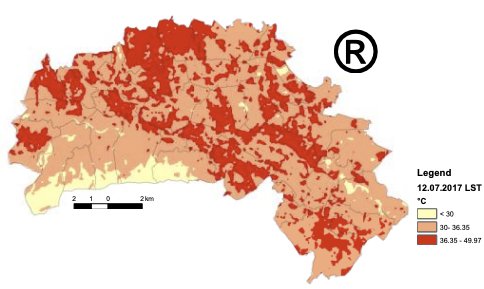
\includegraphics[width=\textwidth]{Includes/1-skopje-LST.png}
            \label{fig:1-skopje-LST}
        \end{minipage}
        \caption{Normalized Difference Vegetation Index \cite{Rouse1973MonitoringVS} and LST measurements for the Skopje, North Macedonia zone. Urban areas with a lower vegetation index tend to have a higher temperature than their rural counterparts (Source: \cite{skopje2018}).} 
        \label{fig:1-skopie-UHI}
    \end{figure}

    Converting the LR images from private constellations into HR images through post-processing techniques like super resolution could enable new frontiers in studying urban heat. 

    \subsection{Irrigation Management}

    Irrigation is typically performed in areas with arid climates and low precipitation. As it uses 70\% of the water used worldwide, proper resource management in those areas is both complex and essential.

    Thermal Remote Sensing, by measuring actual evapotranspiration (ET) and biomass, offers detailed agricultural insights beyond traditional methods like water balance or ground measurements. However, the satellite revisit period of 16 days can lead to significant errors in irrigation performance estimates due to the interpolation done to obtain values between measurements. Uncertainties of up to 40\% in ET calculation have been found compared to revisit periods of 4 days during the rainy season \cite{rs11050573}. 
    The spatial resolution also plays a crucial role in irrigation management, as not all the cropland properties are the same size. Coarser resolutions fail to monitor small to medium land sizes, which constitute around 50\% of the fields in the world \cite{Lesiv2018}. Ororatech's internal estimations say that improving the resolution of FOREST-2 data products by three times would increase the serviceable market by 40\%, from 52\% of the cropland to 72\%. 
    Moreover, ET calculation algorithms were initially developed at high spatial resolutions, usually taken from aerial vehicles, and assume homogeneous conditions across a single pixel. This assumption does not hold at the low spatial resolution data from satellites \cite{rs13081524}.
    In \cite{rs12182949}, the effects of spatial resolution on irrigation performance indicators such as adequacy, equity, and productivity are analyzed, concluding that spatial resolution plays a vital role in the quality of the results. 
    
    Studies have shown that temporal and spatial resolutions are critical in irrigation management. Higher temporal resolution reduces uncertainty in interpolated data, while finer spatial resolution allows for more detailed management decisions and minimizes errors from algorithm assumptions.


    \subsection{The spatio-temporal trade-off}

        Sensors typically trade spatial resolution for temporal resolution, and maximizing both has historically been difficult.
        Sensors with a high spatial resolution often cover a smaller area than those with a lower spatial resolution.
        This is because, with a smaller field of view, it takes longer for a sensor to cover the same area. 

        Essentially, it can be said that currently, the TIR data products that are used for retrieving LST have either: 
        
        \begin{itemize}
            \item High temporal resolution (sub-daily images) but coarse spatial resolution ( in the km range).
            \item High spatial resolution ( $<$ 100 m) but low temporal resolution (several days up to weeks).
        \end{itemize}

        The applications mentioned above have requirements in both spatial and temporal resolution. 
        The zone of interest, composed of sub-daily frequency and a GSD smaller than 100m, is not covered by any existing systems.
        Private missions using smaller satellites can leverage constellations to achieve higher temporal resolution.
        However, the payload mass and energy consumption constraints still limit the spatial resolution.
        This trade-off can be described by displaying the resolution of some of the available LST/TIR data products, as in Fig. \ref{fig:1-spatio-temporal-trade-off}. 

        \begin{figure}[H]
            \centering
            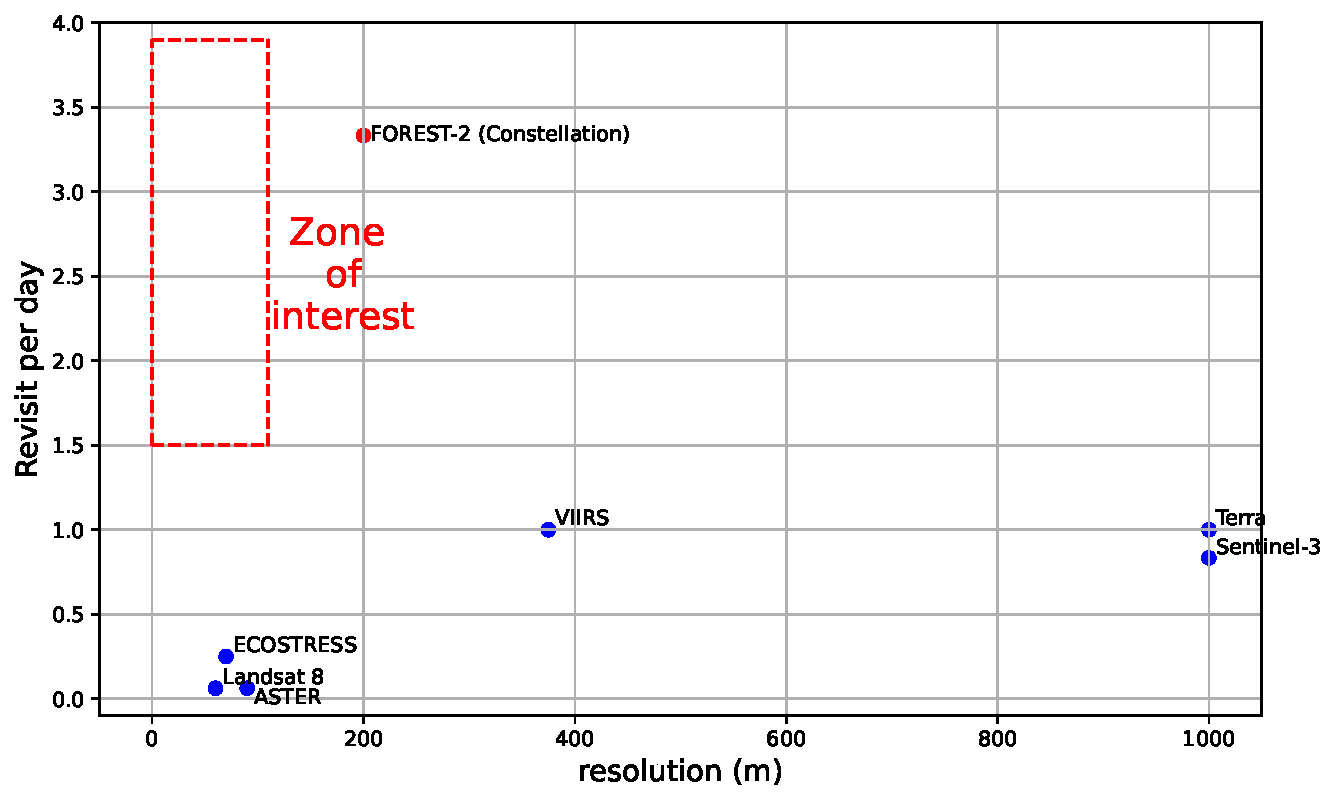
\includegraphics[width=\textwidth]{Includes/2-scatterplot-res-revisit.pdf}
            \caption{Scatter plot of the spatial and temporal resolution of some of the available LST/TIR data products. No mission can provide products in the zone of interest. Constellations may help with temporal resolution, but the spatial resolution is still limited.}
            \label{fig:1-spatio-temporal-trade-off}
        \end{figure}

        This opens the question of whether it is possible to increase the spatial resolution of the data products available using a post-processing technique, such as super resolution, without compromising the physical consistency of the images.
        The main techniques of super resolution and their most complex challenges to apply to LST/TIR data are described in the next section.

\newpage